%%
% Modificación de una plantilla de Latex para adaptarla al castellano.
%%

%%%%%%%%%%%%%%%%%%%%%
% Thin Sectioned Essay
% LaTeX Template
% Version 1.0 (3/8/13)
%
% This template has been downloaded from:
% http://www.LaTeXTemplates.com
%
% Original Author:
% Nicolas Diaz (nsdiaz@uc.cl) with extensive modifications by:
% Vel (vel@latextemplates.com)
%
% License:
% CC BY-NC-SA 3.0 (http://creativecommons.org/licenses/by-nc-sa/3.0/)
%
%%%%%%%%%%%%%%%%%%%%%

%----------------------------------------------------------------------------------------
%	PACKAGES AND OTHER DOCUMENT CONFIGURATIONS
%----------------------------------------------------------------------------------------

\documentclass[a4paper, 11pt]{article} % Font size (can be 10pt, 11pt or 12pt) and paper size (remove a4paper for US letter paper)

\usepackage[protrusion=true,expansion=true]{microtype} % Better typography
\usepackage{graphicx} % Required for including pictures
\usepackage[usenames,dvipsnames]{color} % Coloring code
\usepackage{wrapfig} % Allows in-line images
\usepackage[utf8]{inputenc}
\usepackage{enumerate}
\usepackage{enumitem}

% Imágenes
\usepackage{graphicx} 

\usepackage{amsmath}
% para importar svg
%\usepackage[generate=all]{svgfig}

% sudo apt-get install texlive-lang-spanish
\usepackage[spanish]{babel} % English language/hyphenation
\selectlanguage{spanish}
% Hay que pelearse con babel-spanish para el alineamiento del punto decimal
\decimalpoint
\usepackage{dcolumn}
\newcolumntype{d}[1]{D{.}{\esperiod}{#1}}
\makeatletter
\addto\shorthandsspanish{\let\esperiod\es@period@code}
\makeatother

\usepackage{longtable}
\usepackage{tabu}
\usepackage{supertabular}

\usepackage{multicol}
\newsavebox\ltmcbox

% Para algoritmos
\usepackage{algorithm}
\usepackage{algorithmic}
\usepackage{amsthm}

% Para matrices
\usepackage{amsmath}

% Símbolos matemáticos
\usepackage{amssymb}
\usepackage{accents}
\let\oldemptyset\emptyset
\let\emptyset\varnothing

\usepackage[hidelinks]{hyperref}

\usepackage[section]{placeins} % Para gráficas en su sección.
\usepackage[T1]{fontenc} % Required for accented characters
\newenvironment{allintypewriter}{\ttfamily}{\par}
\setlength{\parindent}{0pt}
\parskip=8pt
\linespread{1.05} % Change line spacing here, Palatino benefits from a slight increase by default

\makeatletter
\renewcommand\@biblabel[1]{\textbf{#1.}} % Change the square brackets for each bibliography item from '[1]' to '1.'
\renewcommand{\@listI}{\itemsep=0pt} % Reduce the space between items in the itemize and enumerate environments and the bibliography
\newcommand{\imagen}[2]{\begin{center} \includegraphics[width=90mm]{#1} \\#2 \end{center}}
\newcommand{\RFC}[1]{\href{https://www.ietf.org/rfc/rfc#1.txt}{RFC-#1}}

\renewcommand{\maketitle}{ % Customize the title - do not edit title and author name here, see the TITLE block below
\begin{center} % Center align
{\Huge\@title} % Increase the font size of the title
\end{center}

\vspace{20pt} % Some vertical space between the title and author name

\begin{flushright} % Right align
{\large\@author} % Author name
\\\@date % Date

\vspace{40pt} % Some vertical space between the author block and abstract
\end{flushright}
}
%----------------------------------------------------------------------------------------
%	TITLE
%----------------------------------------------------------------------------------------

\title{\textbf{Instalación de SO y Configuración de RAID}\\ % Title
\vspace{20 pt}
Ingeniería de Servidores \\Memoria de la Práctica 1} % Subtitle

\author{\textsc{Adrián Portillo Sánchez} % Author
\\{\textit{Universidad de Granada}}} % Institution

\date{\today} % Date

%----------------------------------------------------------------------------------------
\setcounter{secnumdepth}{0}

\begin{document}
\maketitle
\pagebreak
\tableofcontents
\listoffigures
\pagebreak

\section{Cuestión 1}
\textbf{¿Qué modos y/o tipos de “Virtualización” existen?}\\ 
La virtualización es una técnica de simulacion de computadores lógicos o sistemas operativos$^{[1]}$. Esta virtualización puede ser software o hardware, pero como la que vamos a utilizar es la hardware, por lo que nos centraremos en esta. \\La virtualización hardware es el tipo de virtualización más complejo y consiste en emular, haciendo uso de máquinas virtuales, los componentes hardware, por lo que el sistema operativo no se ejecuta sobre un hardware real sino por uno virtual simulado.
\begin{itemize}
\item\textbf{Virtualización Completa:} $^{[2]}$ $^{[3]}$ Esta técnica virtualiza completamente el servidor físico para que este soporte que las aplicaciones y software funcionen de la misma forma que si lo hicieran en la máquina real, así parece que la máquina funciona en un servidor único. Este sistema permite virtualizar diferentes sistemas operativos de distintas plataformas sin necesidad de alterarlos, ya que algunos Sistemas Operativos están diseñados para funcionar en la misma arquitectura que el anfitrión.
\item\textbf{Virtualización con host:} $^{[2]}$ $^{[4]}$ Esta técnica es la que se utiliza en las máquinas virtuales que usamos normalmente, como VMWare o VirtualBox, se instala una capa de virtualización encima del sistema operativo host, entonces los sistemas operativos invitados se instalan encima del nivel de virtualización. La máquina virtual simula multiples instancias compuestas en su mayoria por un entorno hardware, en especial los espacios de direcciones, no todo el sistema operativo podrá funcionar en estas máquinas pero si muchas de sus aplicaciones.  
\item\textbf{Paravirtualización:} $^{[1]}$ $^{[4]}$ No es necesario simular el hardware, consisten en ejecutar sistemas operativos huéspedes (guest) sobre otro sistema operativo anfitrión (funciona como un Hipervisor), los SO huesped se comunican con el hipervisor para lograr la virtualización, requiere modificar el Sistema Operativo invitado.
\end{itemize}

\pagebreak 

\section{Cuestión 2}
\textbf{Busque en Internet ofertas de servicios de varios proveedores de VPS (Virtual Private Server) y compare con el precio de alquiler del servicio, con el de uso de servidores dedicados (administrados y no administrados) de características similares.}\\ \\

\textbf{Proveedor: Bluehost.com}\\
$^{[2]}$ Coste de Virtual Private Server: 119.99\$\\
$^{[1]}$ Coste de Servidor Dedicado (administrado): 149.99\$\\
\begin{table}[h]
	\begin{tabular}{|c|c|c|}
	\hline 
	Bluehost.com & VPS & Dedicated Server \\ 
	\hline 
	CPUs & 4 & 4 \\ 
	\hline 
	Capacidad& 240GB & 1TB(mirrored) \\ 
	\hline 
	RAM & 8GB & 4GB \\ 
	\hline 
	Ancho de banda & 4TB & 5TB \\ 
	\hline 
	Dominios & 1 & 1 \\ 
	\hline 
	Direcciones IP & 2 & 3 \\ 
	\hline 
	Administración & 24/7 & 24/7 \\ 
	\hline 
	\end{tabular}
\end{table} 

\textbf{Proveedor: Inmotionhosting.com}\\
$^{[3]}$ Coste de Virtual Private Server: 74.99\$\\
$^{[4]}$ Coste de Servidor Dedicado (administrado): 219.99\$\\
\begin{table}[h]
	\begin{tabular}{|c|c|c|}
	\hline 
	Inmotionhosting.com & VPS & Dedicated Server \\ 
	\hline 
	CPUs & No especificado & 4 (+Hyperthreading) \\ 
	\hline 
	Capacidad& 130GB & 128GB SSD/1TB HDD \\ 
	\hline 
	RAM & 8GB & 8GB \\ 
	\hline 
	Ancho de banda & 4TB & 10TB \\ 
	\hline 
	Direcciones IP & 3 & 15 \\ 
	\hline 
	Administración & Control panel & Control Panel \\ 
	\hline 
	\end{tabular}
\end{table} 

\section{Cuestión 3}
\textbf{¿Qué otros software de virtualización existen además de VMWare y Virtual Box?} \\
\begin{itemize}
\item \textbf{Parallels desktop:}
	$^{[1]}$ $^{[2]}$ Se trata de un sistema de Virtualización de Hardware, en la que cada máquina virtual funciona de manera independiente con prácticamente todos los recursos de un equipo físico, una gran ventaja es el uso compartido de controladores que fomenta la portabilidad de las MV de un equipo a otro, la principal diferencia con VMware y VirtualBox es que está pensada para equipos Mac y por tanto lo convierte en un software util para los que usan Mac OS X.
\item \textbf{CoLinux:}
	$^{[3]}$ $^{[4]}$ La principal característica de CoLinux es que es un software que permite ejecutar de forma paralela Microsoft Windows y Linux, esto lo consigue haciendo uso de CVM o Cooperative Virtual Machine, que consiste en compartir los recursos que ya existen en el sistema operativo. Es distinto de otras soluciones como VMware o VirtualBox pues que normalmente estos trabajan para hacer funcionar el SO huésped con un menor privilegio que el anfitrión, pero CoLinux tiene desventajas como la seguridad o bién la estabilidad ya que depende en gran medida del SO anfitrión.
\end{itemize}

\section{Cuestión 4}
\textbf{Enumere algunas innovaciones en Windows 2012 R2 respecto a 2008 R2. $^{[1]}$} \\
\begin{itemize}
\item \textbf{Control de acceso dinámico:} $^{[2]}$ Los permisos de acceso se pueden configurar y asignar de forma dinámica, es decir, se pueden aplicar permisos y restricciones de acuerdo a reglas definidas sobre los recursos, el usuario o la configuración del dispositivo.
\item \textbf{Bajo coste, y almacenamiento de archivos basados en alta disponibilidad:} Windows server 2012 introduce SMB 3.0 un protocolo de red que permite compartir archivos entre otros equipos de una red.
\item \textbf{Virtualización de red (Hiper-V):} Windows server 2012 tiene la capacidad de aislar el tráfico de la red  de diferentes unidades que están ocupadas.
\item \textbf{Permite migrar máquinas virtuales} entre host que usen Hiper-V en diferentes clusters o servidores sin almacenamiento compartido.
\item \textbf{Windows PowerShell 3.0} tiene una notable mejora en la versión 2012 puesto que soporta más de 2300 command-lets, son scripts que realizan diversas funcionalidades.
\end{itemize}

\section{Cuestión 5}
\textbf{¿Qué empresa hay detrás de Ubuntu? ¿Qué otros productos/servicios ofrece?}\\ 
Tras ubuntu se encuentra la empresa Canonical, $^{[1]}$: \textit{''Compañía britanica propiedad del empresario Mark Shuttleworth''.} \\ \\$^{[2]}$ $^{[3]}$ Ofrece productos como: Ubuntu para teléfonos y tablets, Ubuntu TV, Ubuntu One (Un servidor de archivos), Ubuntu Cloud, Mir o Launchpad (Un servidor gráfico) , y otros servicios como JuJu o MAAS (Un servicio que se encarga de tomar servidores físicos que se podrán usar
en demanda.)\\


\section{Cuestión 6}
\textbf{¿Qué relación tiene esta distribución con Red Hat y con el proyecto Fedora?}\\ 
$^{[1]}$ $^{[2]}$ Fedora es el proyecto principal de Workstation de Red Hat$^{\circledR}$ y está basado en comunidad, es decir, las distribuciones son gratuitas centradas en sacar rápidas versiones con nuevas funcionalidades. \\Ahora bién, Red Hat Enterprise Linux está basado en Fedora, solo que se trata de una versión comercial y no es gratuito puesto que viene con soporte para sus distribuciones y se centra en sacar versiones más estables de sus productos. \\Por último, CentOS es básicamente la versión de comunidad de RHEL con la diferencia de que es gratuita puesto el soporte viene proporcionado por la misma comunidad.

\pagebreak

\section{Cuestión 7}
\textbf{Busque indicadores de porcentaje de uso global o de cuota de mercado de SO de Servidores. No olvide poner la fuente de donde saca la información y preste atención a la fecha de ésta.}\\
$^{[1]}$ $^{[2]}$ $^{[3]}$ Según esta fuente de información (actualizada el mismo 25 de Octubre de 2015) el porcentaje de uso global de los sistemas operativos es:
\begin{itemize}
\item \textbf{UNIX:} 67.3\%
	\begin{itemize}
	\item \textbf{Linux:} 53.1\%
	    \begin{itemize}
	    \item[-] Debian: 31.7\%
        \item[-] Ubuntu: 30.1\%
        \item[-] CentOS: 20.7\%
        \item[-] Red Hat: 4.2\%
        \item[-] Gentoo: 2.2\%
        \item[-] Fedora: 1.3\%
        \item[-] SuSE: 1.1\%
        \item[-] Scientific Linux: 0.1\%
        \item[-] Turbolinux: 0.1\%
        \item[-] Mandriva: 0.1\%
        \item[-] CloudLinux: menos de 0.1\%
        \item[-] Asianux: menos de 0.1\%
        \item[-] Mageia: menos de 0.1\%
        \item[-] StartCom Linux: menos de 0.1\%
        \item[-] PLD Linux: menos de 0.1\%
        \item[-] Desconocido: 8.4\%
	    \end{itemize}
	\item BSD: 1.3\%
	\item Darwin: menos de 0.1\%
	\item HP-UX: menos de 0.1\%
	\item Solaris: menos de 0.1\%
	\item Desconocido: 45.6\%
	\end{itemize}
\item \textbf{Windows:} 32.7\%
\end{itemize}

\pagebreak

\section{Cuestión 8}
\textbf{¿Qué diferencia hay entre RAID mediante SW y mediante HW?}\\

$^{[1]}$ En el RAID por Hardware el sistema hardware es el que gestiona el conjunto de discos independientemente del sistema de la máquina, a través de un controlador específico, y presenta a la máquina el conjunto de discos RAID como si se tratara de un único disco. Este controlador es una tarjeta que controla todas las comunicaciones del disco con el sistema, que son bastante caras; por lo que aunque esta alternativa es mejor funcionalmente y es la que se suele usar en servidores también se tiene en cuenta otra alternativa, el RAID por Software. \\
El RAID por Software, a pesar de eso, es más barato; en él los diversos niveles del RAID se implementan en el código del Kernel, y el controlador en lugar de situarse en una tarjeta independiente del sistema, pasa a formar parte del sistema, por lo que consume recursos de este.


\section{Cuestión 9}
\textbf{a) ¿Qué es LVM? b)¿Qué ventaja tiene para un servidor de gama baja? c) Si va a tener un servidor web, ¿le daría un tamaño grande o pequeño a /var?}\\ 
\begin{itemize}
\item[a)]$^{[1]}$ LVM(lógical Volumes Manager) o administrador de volúmenes lógicos sirve para el kernel de linux que gestiona unidades de disco y dispositivos de almacenamiento masivo, además hace posible crear un espacio de almacenamiento abstracto, por lo que es más facil aumentar o disminuir el tamaño de las particiones y eliminar o crear particiones evitando problemas de posicionamiendo.
\item[b)] $^{[2]}$ El particionamiento del disco en GNU/Linux es uno de los grandes problemas puesto que si se realiza sin LVM el esquema de particionado que se haya establecido no es sencillo de redimensionar normalmente es necesario reformatear para cambiar dicho esquema, entonces la ventaja de LVM es que si tienes un esquema de particionamiento y algunas de las particiones se llenan, es posible una redimensión puesto que son particiones lógicas, y esto puede beneficiar a los servidores cuyas particiones se vean sin capacidad puesto que se usaría espacio de otras que estén libres para aumentar el tamaño.
\item[c)] La carpeta ''/var'' tiene información de datos que cambian al ejecutarse el sistema, en el caso de un servidor web precisamente se trata con ''/var/www'', pienso que si el sistema no usa LVM el espacio para ''/var/'' debe ser grande ya que como la información va cambiando puede cambiar mucho el tamaño y si es pequeño necesitaras realizar una limpieza o formatearlo para redimensionar; en el caso de que el sistema use LVM la asignación tendrá que ser más o menos adecuada para que no haya que redimensionar demasiado pronto, pero como se puede no es necesario asignar un tamaño muy grande en un inicio. 
\end{itemize}

\section{Cuestión 10}
\textbf{¿Debemos cifrar también el volumen que contiene el espacio para swap? ¿y el volumen en el que montaremos /boot?
}\\ 
$^{[1]}$  Si es conveniente para proteger datos que se intercambian desde memoria, como ejemplo una aplicación que haga uso de passwords mientras se encuentren en memoria serán limpiadas de la misma despues de un reinicio, pero es posible que el sistema operativo empiece a intercambiar con el disco dichas passwords con el objetivo de liberar memoria para otras aplicaciones, y al no estar encriptado swap sería posible acceder a ellas.
\\$^{[2]}$  No es posible cifrar el volumen en el que se monta /boot puesto que no se puede arrancar desde un volumen cifrado, y por tanto es necesario una partición que no este encriptada para el arranque. $^{[3]}$Es el paquete LUKS el que permite el cifrado y descifrado de particiones, y este no puede funcionar desde el MBR, es decir, sin que arranque el sistema no es posible que este paquete funcione.

\section{Cuestión 11}
\textbf{¿Cuál es la diferencia más significativa entre ext4 y ext2?}\\
$^{[1]}$ La diferencia más importante entre ext2 y ext4 es que ext4 usa registro por diario o "journaling", que se puede desactivar, es un registro que almacena la información que sirve para restablecer datos dañados; además otra diferencia muy importante es que usa un árbol AVL. Un dato importante es que ext4 se puede usar como si fuera ext2.  El tamaño máximo de archivos individuales en ext2 es de entre 16GB y 2TB mientras que en ext4 entre 16GB y 16TB. El tamaño máximo de disco en ext2 es de entre 2TB y 32TB, mientras que en ext4 es de 1EB

\pagebreak

\section{Cuestión 12}
\textbf{Muestre cómo ha quedado el disco particionado una vez el sistema está instalado.}\\
\begin{figure}[h]
\centering 
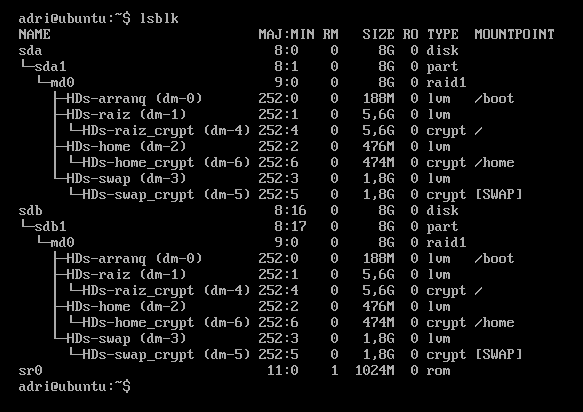
\includegraphics[width=1\linewidth]{lsblk.png} 
\caption{Particiones de disco del sistema.} 
\label{contexto:figura} 
\end{figure}


\section{Cuestión 13}
\textbf{a) ¿Cómo ha hecho el disco 2 “arrancable”? b) ¿Qué hace el comando grub-install? c) ¿Qué hace el comando dd?} \\ 

El segundo disco se puede hacer arrancable (bootable) haciendo uso de la orden: "\textit{grub-install /dev/sdb}" donde sdb es el segundo disco tal y como podemos apreciar en la figura anterior. $^{[1]}$Grub-install instala grub en un dispositivo, y $^{[2]}$ grub es un gestor de arranque que ha sido desarrollado por GNU y permite iniciar con distintos sistemas operativos en un mismo equipo.\\
$^{[3]}$ El comando dd (Dataset Definition) se utiliza sobre dispositivos: discos y particiones con la orden "\textit{sudo dd if=origen of=destino}'' y permite copiar todos los datos y configuraciones de un dispositivo de origen a otro de destino, creando una copia completa del dispositivo de origen en el de destino, entre otras cosas permite crear copias de seguridad, .isos, copias de datos, etc.

\section{Cuestión Opcional 1}

\textbf{Muestre (con capturas de pantalla) cómo ha comprobado que el RAID1 funciona.$^{[1]}$}\\ 

\begin{itemize}
\item Primero creamos unos archivos en el disco para comprobar luego que permanecen ahí.

\begin{figure}[h]
\centering 
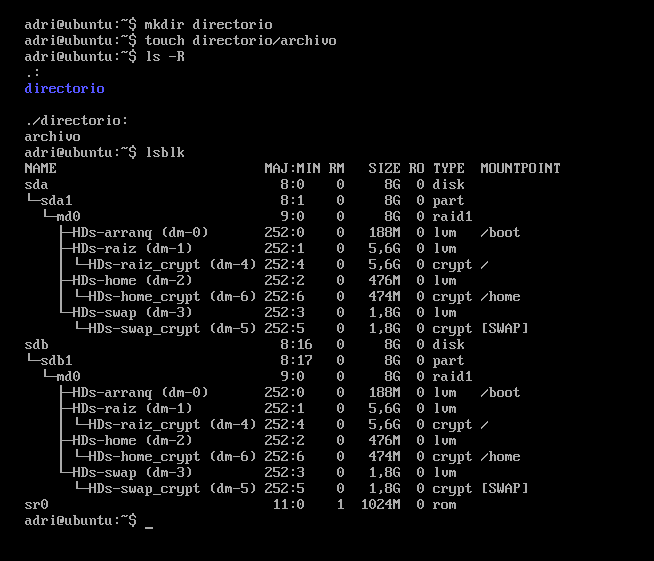
\includegraphics[width=1\linewidth]{comprobacion1.png} 
\caption{Creando archivos.} 
\label{contexto:figura} 
\end{figure}

\pagebreak

\item Luego forzamos un error en el disco 1 (sda), de la siguiente forma:

\begin{figure}[h]
\centering 
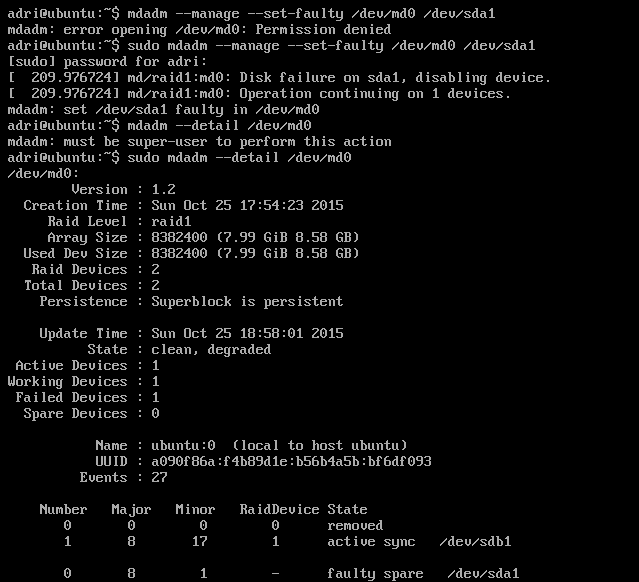
\includegraphics[width=1\linewidth]{comprobacion2.png} 
\caption{Provocando un error en el disco 1.} 
\label{contexto:figura} 
\end{figure}

\item Podemos ver que tras el error dice: "\textit{operation continuing on 1 devices}", lo cual quiere decir que nuestro RAID funciona correctamente, ya que el sistema se sigue ejecutando en el otro disco duro.

\pagebreak

\item Comprobamos que nuestros archivos siguen ahí, desconectamos el disco (como se muestra en la figura) y volvemos a comprobar:

\begin{figure}[h]
\centering 
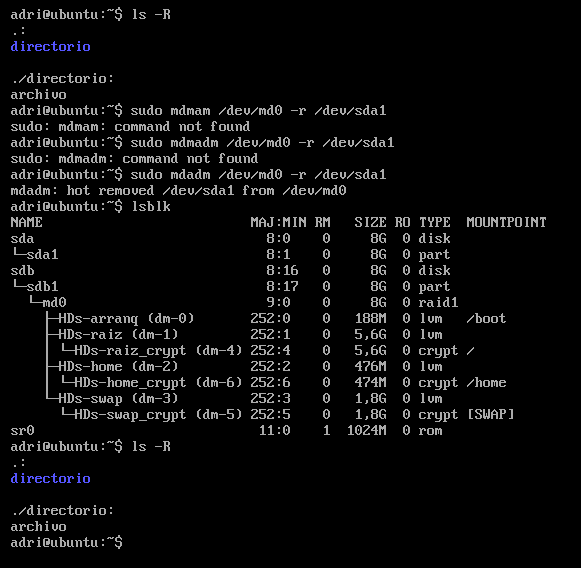
\includegraphics[width=1\linewidth]{comprobacion3.png} 
\caption{Desconectando el disco 1.} 
\label{contexto:figura} 
\end{figure}

\pagebreak

\item Volvemos a añadir el disco y comprobamos que todo está correcto:

\begin{figure}[h]
\centering 
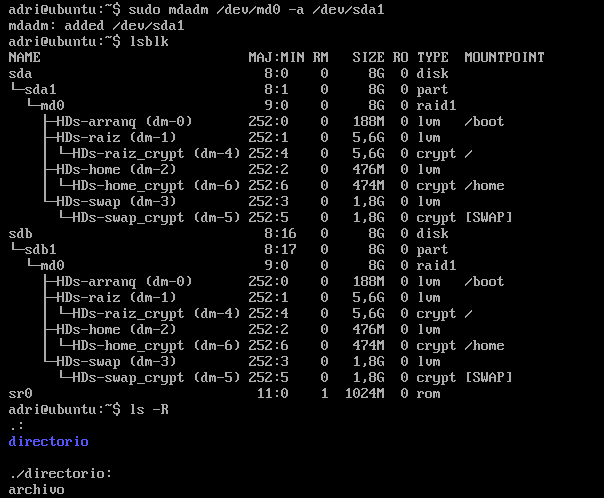
\includegraphics[width=1\linewidth]{comprobacion4.png} 
\caption{Reconectando el disco 1.} 
\label{contexto:figura} 
\end{figure}

\pagebreak

\begin{figure}[h]
\centering 
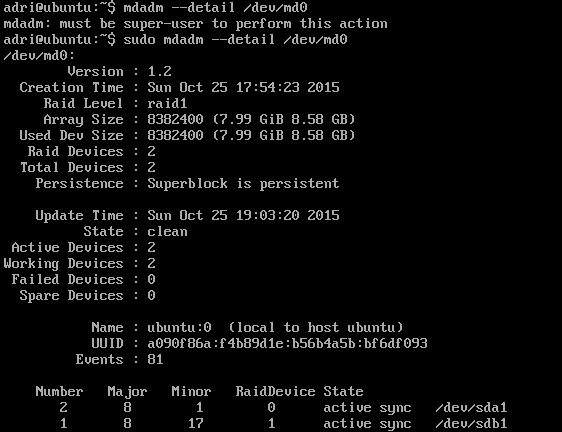
\includegraphics[width=1\linewidth]{comprobacion5.png} 
\caption{Comprobando que todo funciona correctamente.} 
\label{contexto:figura} 
\end{figure}

\end{itemize}


\section{Cuestión 14}
\textbf{¿Cuál es la principal diferencia hay entre las versiones Standard y Datacenter de Windows 2012?}\\
$^{[1]}$ La principal diferencia es el número de máquinas virtuales que se le permite al usuario usar, en la versión Standard se pueden llegar a usar hasta 2 MVs mientras en la versión Datacenter se pueden ejecutar un número ilimitado de ellas, además como dato las licencias de ambas versiones cubren hasta dos procesadores físicos.

\pagebreak

\section{Cuestión 15}
\textbf{Continúe usted con el proceso de definición de RAID1 para los dos discos de 50MiB que ha creado. Muestre el proceso con capturas de pantalla.}\\ \\
$^{[1]}$En primer lugar creamos los nuevos discos, nos dirigimos al administrador de equipo y vemos los dos nuevos discos sin asignar. Tenemos que hacer los discos dinámicos por lo cual seleccionaremos la opción en el disco 1 "\textit{Convertir a dinámico}", después creamos un nuevo volumen simple y agregamos su reflejo, así tendremos configurado el RAID 1. 

\begin{figure}[h]
\centering 
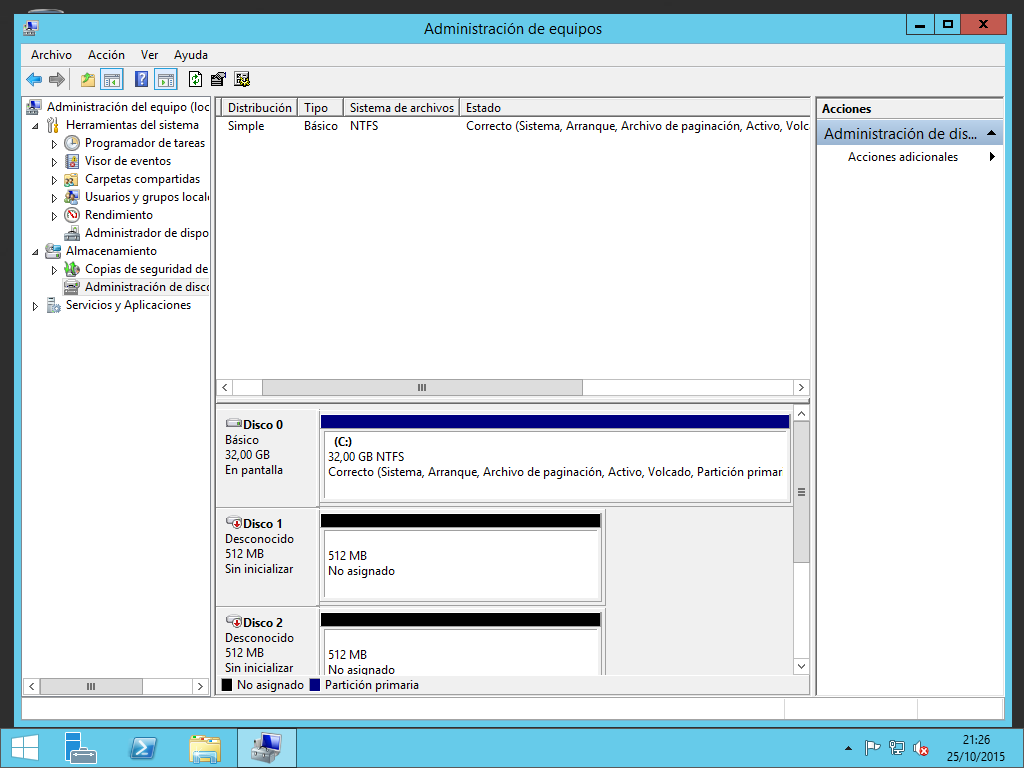
\includegraphics[width=1\linewidth]{instalacion1.png} 
\caption{Estado inicial de los discos.} 
\vspace{-0.5cm}
\label{contexto:figura} 
\end{figure}

\pagebreak
Ponemos los discos en línea e inicializamos los dos discos con tabla de particiones sencilla (ambas opciones mediante el click derecho), y convertimos los dos discos en discos dinámicos:

\begin{figure}[h]
\centering 
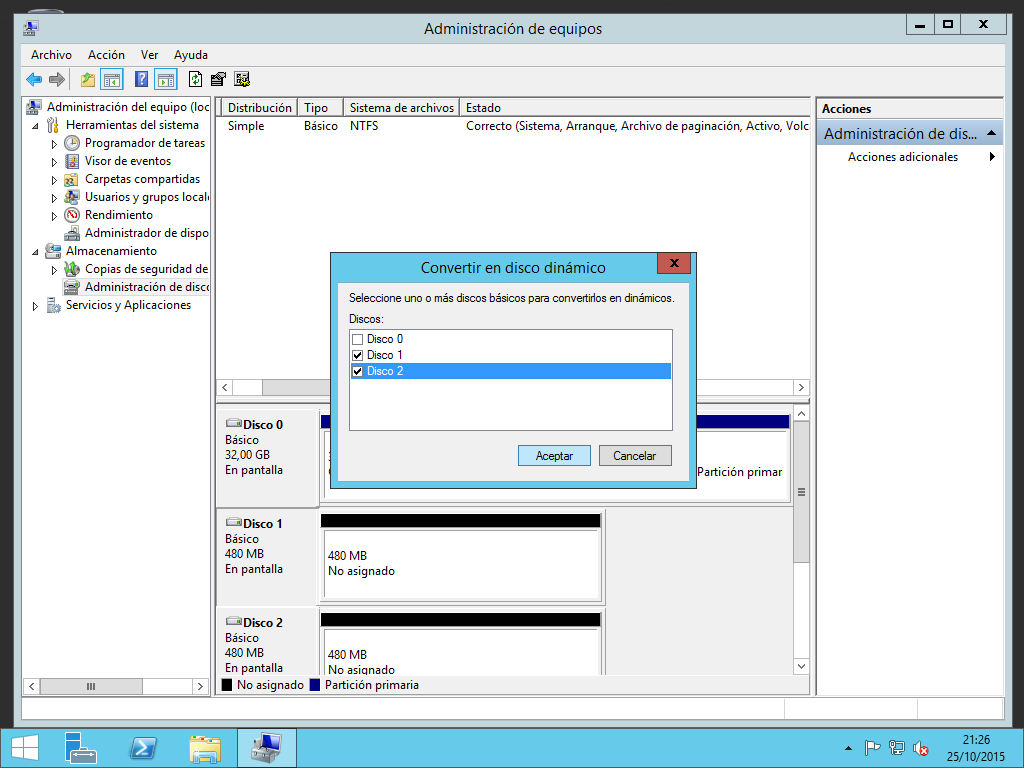
\includegraphics[width=1\linewidth]{instalacion2.png} 
\caption{Pasando los discos a dinámicos.} 
\vspace{-0.2cm}
\label{contexto:figura} 
\end{figure}

\pagebreak
Ponemos uno de los discos como nuevo volumen reflejado:

\begin{figure}[h]
\centering 
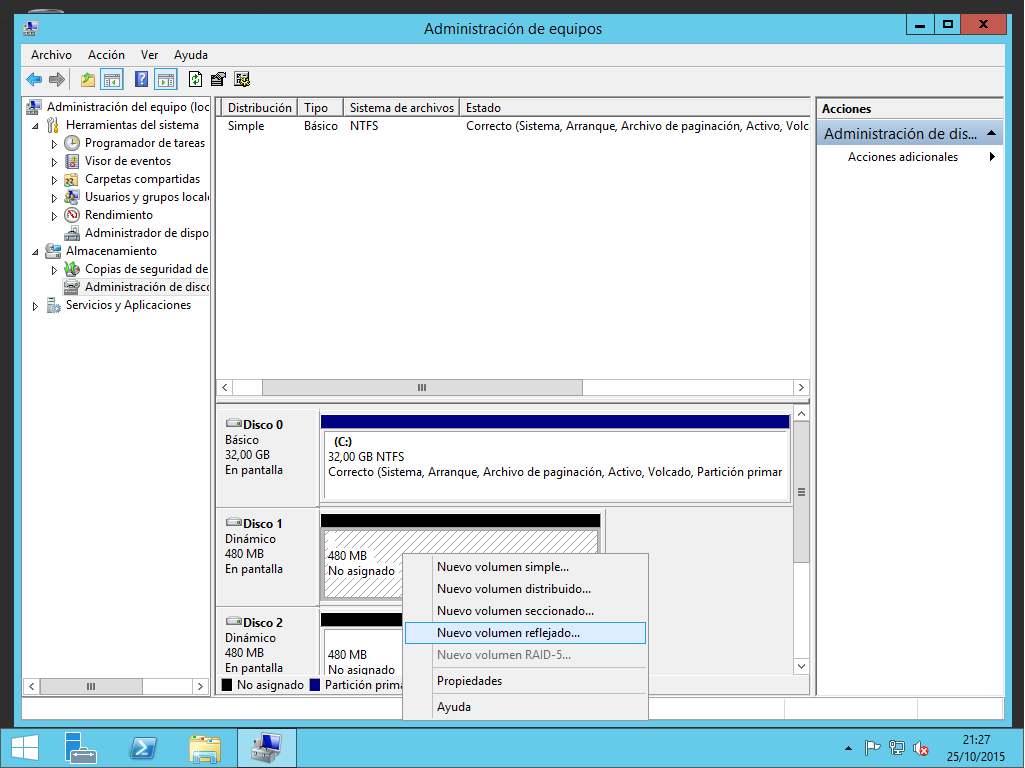
\includegraphics[width=1\linewidth]{instalacion3.png} 
\caption{Creando nuevos volúmenes reflejados.} 
\label{contexto:figura} 
\end{figure}

\pagebreak
Añadimos el segundo disco al volumen reflejado y le asignamos la letra que queramos: 

\begin{figure}[h]
\centering 
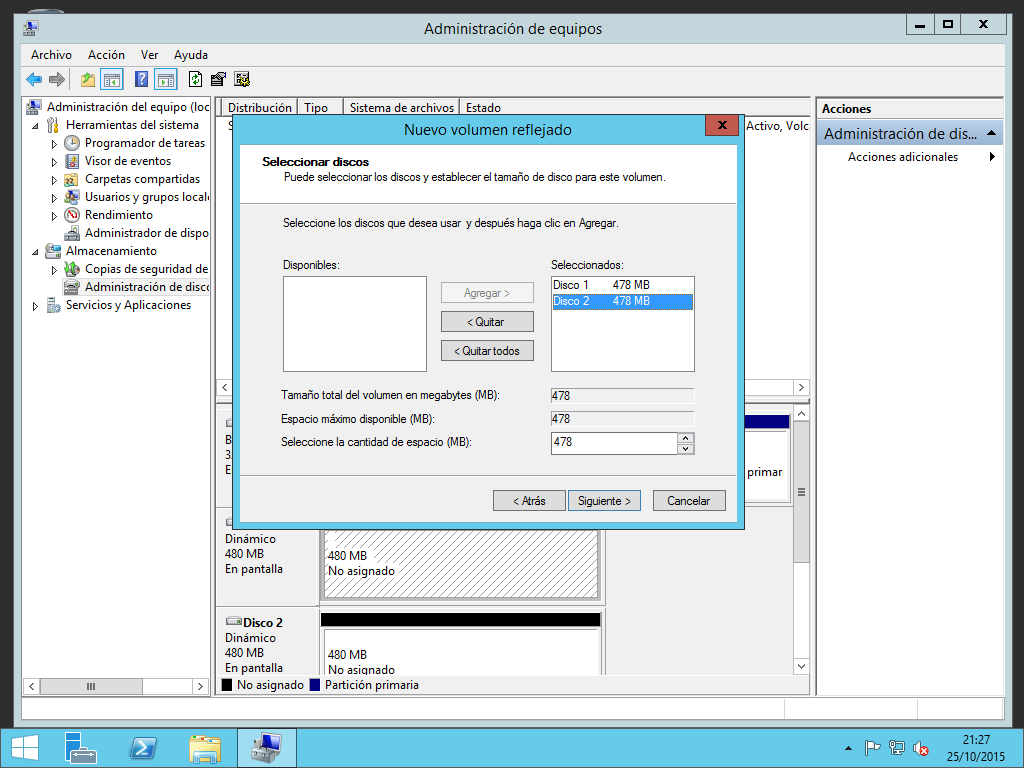
\includegraphics[width=1\linewidth]{instalacion4.png} 
\caption{Agregamos el segundo disco al bloque de discos reflejados.} 
\vspace{-0.2cm}
\label{contexto:figura} 
\end{figure}

\pagebreak
Formateamos el disco con el formato de archivo que queramos y le damos un nombre al RAID:

\begin{figure}[h]
\centering 
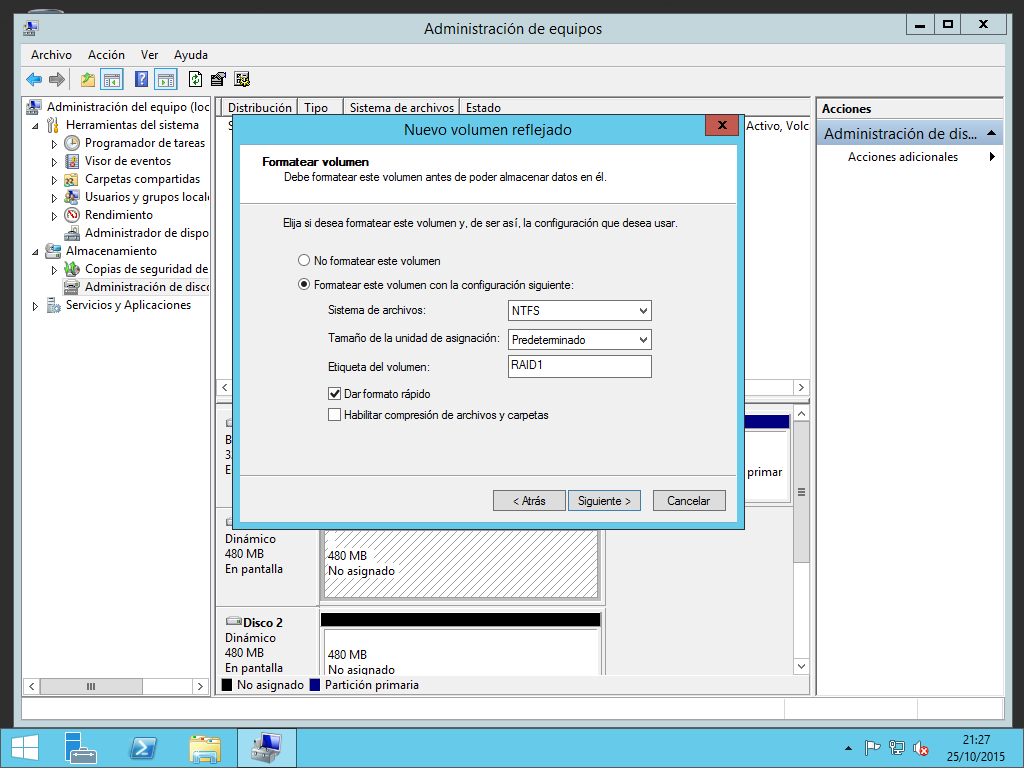
\includegraphics[width=1\linewidth]{instalacion5.png} 
\caption{Seleccionando las opciones de formateo.}
\vspace{-0.2cm} 
\label{contexto:figura} 
\end{figure}

\pagebreak
Así deberá ser el resultado final:

\begin{figure}[h]
\centering 
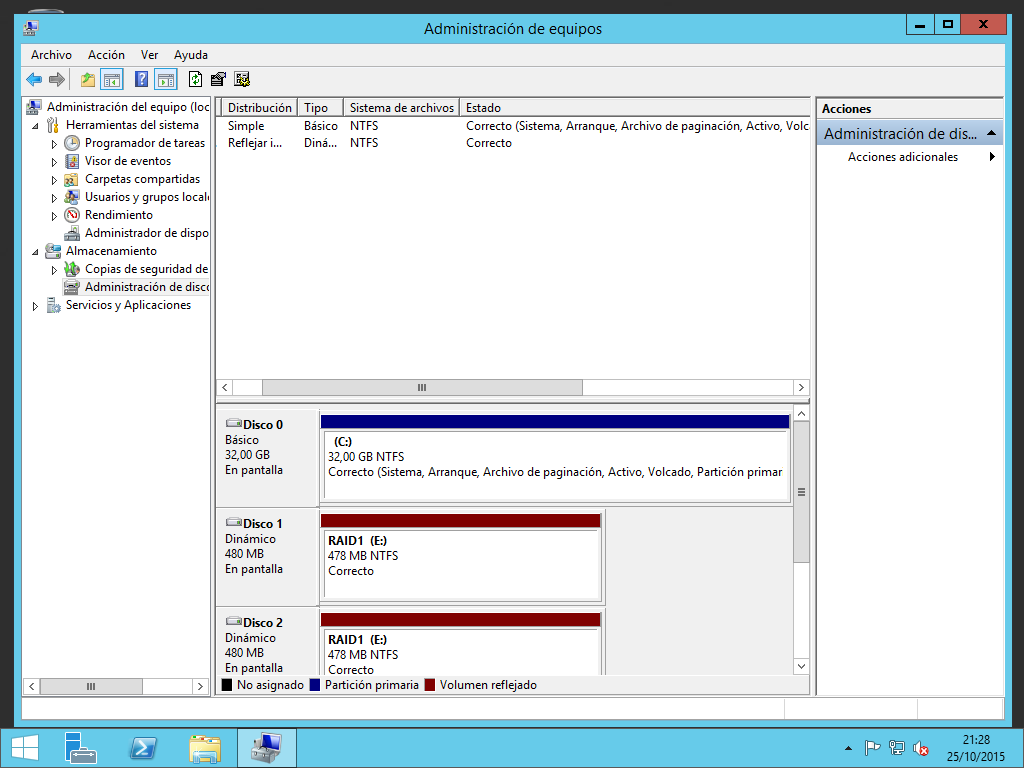
\includegraphics[width=1\linewidth]{instalacion6.png} 
\caption{Estado final del RAID 1.}
\vspace{-0.2cm} 
\label{contexto:figura} 
\end{figure}

\section{Cuestión 16}
\textbf{Explique brevemente qué diferencias hay entre los tres tipos de conexión que permite el VMSW para las Mvs: NAT, Host-only y Bridge.$^{[1]}$}
\begin{itemize}
\item \textbf{NAT: } $^{[2]}$En el modo NAT (Network Adress Translation) se crea una red virtual aislada del resto de equipos de la red local, y la conexión de la MV a la red se realiza a través de un switch virtual que crea la aplicación de virtualización, creando una conexión de red entre el anfitrión y un switch virtual. La red de la máquina virtual pasa a formar parte de la red del equipo físico, y tiene acceso a la misma extensión de red que la máquina anfitriona.
\item \textbf{Bridge: }Bridge es una extensión de la red sin necesidad de utilizar otro router, la máquina virtual se conectará a la red como si fuera un equipo más de la red; la red local se extiende hacia la MV. \\ \\
\item \textbf{Host-only: }En el modo host-only, la red de la máquina virtual se aísla completamente de la red local, y por tanto la red de la máquina virtual sólamente llega al equipo que la esté utilizando.
\end{itemize}

\section{Cuestión Opcional 2}
\textbf{¿Qué relación hay entre los atajos de teclado de emacs y los de la consola bash? ¿y entre los de vi y las páginas del manual?}\\

$^{[1]}$En el modo bash-emacs, la navegación con cursor es la misma que la navegación con teclado en emacs.
\begin{description}
\item [CTRL-P:] Volverá a un comando anterior en bash, y se moverá a la linea superior en emacs.
\item [CTRL-B:] Moverá atrás un carácter (bash y emacs)
\item [CTRL-F:] Moverá adelante un carácter (bash y emacs)
\end{description}
Y así para todos los relacionados con la navegación del cursor.\\ \\
$^{[2]}$En el manual de Linux y en vi tenemos atajos similares para facilitar la navegación:
\begin{itemize}
\item Si pulsas / y escribes algo que quieras buscar y pulsas enter. Te mostrará el primer resultado. Puedes pulsar n para pasar al siguiente y Shift+n para volver.
\item Puedes usar marcadores para guiarte en documentos muy largos, para ello pulsas 'm' y una tecla, y entonces la próxima vez que pulses 'a' y esa misma tecla volverás a esa posición del documento.
\item Puedes usar 'd' y 'u' para avanzar media página arriba o abajo.
\end{itemize}
también puedes usar vi para leer archivos del manual con la línea "man [Artículo de man] | vi -".


\pagebreak
\begin{thebibliography}{X}
\bibitem{Baz} Cuestión 1:\\ 
 \textbf{1.}\url{https://blog.smaldone.com.ar/2008/09/20/virtualizacion-de-hardware/ }\\
 \textbf{2.}\url{http://vmblog.com/archive/2012/04/30/types-of-hardware-virtualization-techniques-and-its-advantages.aspx#.VjEHh6rYUvQ}\\
 \textbf{3.}\url{https://openwebinars.net/introduccion-la-virtualizacion/}
 \textbf{4.}\url{https://technet.microsoft.com/es-es/magazine/hh802393.aspx}
\bibitem{Baz} Cuestión 2:\\ 
 \textbf{1.}\url{http://www.bluehost.com/dedicated}\\
 \textbf{2.}\url{http://www.bluehost.com/vps}\\
 \textbf{3.}\url{https://www.inmotionhosting.com/vps-hosting}\\
 \textbf{4.}\url{https://www.inmotionhosting.com/dedicated-servers}
\bibitem{Baz} Cuestión 3:\\
 \textbf{1.}\url{http://es.wikipedia.org/wiki/Parallels_Desktop_para_Mac#Caracter.C3.ADsticas_T.C3.A9cnicas}\\
 \textbf{2.}\url{http://www.parallels.com/es/products/desktop/}\\
 \textbf{3.}\url{http://es.wikipedia.org/wiki/Cooperative_Linux#Hardware_emulado}\\
 \textbf{4.}\url{http://www.colinux.org/}
\bibitem{Baz} Cuestión 4:\\
	\textbf{1.}\url{http://www.microsoft.com/en-us/download/details.aspx?id=41703}
	\textbf{2.}\url{https://technet.microsoft.com/es-es/library/jj134043.aspx}
\bibitem{Baz} Cuestión 5:\\
	\textbf{1.}\url{http://es.wikipedia.org/wiki/Canonical}\\
	\textbf{2.}\url{http://www.canonical.com/products}\\
	\textbf{3.}\url{http://www.canonical.com/services}
\bibitem{Baz} Cuestión 6:\\
	\textbf{1.}\url{https://danielmiessler.com/study/fedora_redhat_centos/}\\
	\textbf{2.}\url{http://es.wikipedia.org/wiki/CentOS}
\bibitem{Baz} Cuestión 7:\\
	\textbf{1.}\url{http://w3techs.com/technologies/overview/operating_system/all}\\
	\textbf{2.}\url{http://w3techs.com/technologies/details/os-unix/all/all}\\
	\textbf{3.}\url{http://w3techs.com/technologies/details/os-linux/all/all}
\bibitem{Baz} Cuestión 8:\\
	\textbf{1.}\url{http://web.mit.edu/rhel-doc/3/rhel-sag-es-3/s1-raid-approaches.html}
\bibitem{Baz} Cuestión 9:\\
	\textbf{1.}(Cambiar -n- por ñ)\url{https://wiki.archlinux.org/index.php/LVM_(Espa-n-ol)#Bloques_para_construir_LVM}\\
	\textbf{2.}\url{http://glatelier.org/2010/01/19/lvm-en-gnulinux-parte-i-que-es-y-a-quien-le-sirve/}
\bibitem{Baz} Cuestión 10:\\
	\textbf{1.}\url{http://askubuntu.com/questions/313564/why-encrypt-the-swap-partition}\\
	\textbf{2.}\url{http://byte-inside.blogspot.com.es/2011/09/la-paranoia-full-encriptando-discos-lvm.html}\\
	\textbf{3.}\url{http://www.alcancelibre.org/staticpages/index.php/ciframiento-particiones-luks}
\bibitem{Baz} Cuestión 11:\\
	\textbf{1.}\url{http://www.thegeekstuff.com/2011/05/ext2-ext3-ext4/}
\bibitem{Baz} Cuestión 13:\\
	\textbf{1.}\url{http://linux.die.net/man/8/grub-install}\\
	\textbf{2.}\url{http://es.wikipedia.org/wiki/GNU_GRUB}\\
	\textbf{3.}\url{http://blog.desdelinux.net/uso-del-comando-dd/}
\bibitem{Baz} Cuestión 14:\\
	\textbf{1.}\url{http://www.internetya.co/windows-server-2012-ediciones-datacenter-y-standard/}
\bibitem{Baz} Cuestión 15:\\
	\textbf{1.}\url{https://www.youtube.com/watch?v=j1fNfSxfEuQ}
\bibitem{Baz} Cuestión 16:\\
	\textbf{1.}\url{http://monzisez.blogspot.com.es/2010/09/modo-bridge-host-only-y-nat-explicado.html}\\
	\textbf{2.}\url{http://miguelzunda-redes.blogspot.com.es/2015/04/vmware-adaptador-de-red-que-es-el-modo_19.html}
\bibitem{Baz} Cuestión opcional 1:\\
	\textbf{1.}\url{https://raid.wiki.kernel.org/index.php/Detecting,_querying_and_testing}
\bibitem{Baz} Cuestión opcional 2:\\
	\textbf{1.}\url{http://unix.stackexchange.com/questions/238335/relation-between-emacs-and-bash-terminal-shortcuts}\\
	\textbf{2.}\url{http://stackoverflow.com/questions/22342566/how-to-read-linux-man-pages/28151693#28151693}
\end{thebibliography}


\end{document}